%%%%%%%%%%%%%%%%%%%%%%%%%%%%%%%%%%%%%
%%%%%%%%%% Plantilla del Team para el proyecto final 
%%%%%%%%%%%%%%%%%%%%%%%%%%%%%%%%%%%%%
%%%%%%%%%% Nueva clase personalizada
\documentclass{staprojteamusb}
%%%%%%%%%% Nuevo estilo personalizado
\usepackage{staprojteamusbsty}

\addbibresource{referencias.bib}
%%%%%%%%%%%%%%%%%%%%%%%%%%%%%%%%%%%
%%%%%%%%%% Variables de Markdown
%%%%%%%%%%%%%%%%%%%%%%%%%%%%%%%%%%%
%%%%%%%%%% Encabezado 
\titulo{Análisis estadístico sobre una base de datos de beísbol.}

\autor{
		Eduardo Gavazut\\
	Universidad Simón Bolívar \\
	Caracas, Venezuela \\
	\texttt{\href{mailto:13-10524@usb.ve}{\nolinkurl{13-10524@usb.ve}}} \\
	 \And
		Luis Riera\\
	Universidad Simón Bolívar \\
	Caracas, Venezuela \\
	\texttt{\href{mailto:16-10976@usb.ve}{\nolinkurl{16-10976@usb.ve}}} \\
	 \And
		Miguel Cordero\\
	Universidad Simón Bolívar \\
	Caracas, Venezuela \\
	\texttt{\href{mailto:15-10326@usb.ve}{\nolinkurl{15-10326@usb.ve}}} \\
	}
\fecha{8 de abril de 2022}
\resumen{En este documente se muestran los gráficos de dispersión, y
matriz de correlación entre cada una de las variables. Aún se está
desarrollando}

\palabrasc{Proyecto, Estadistica, Rstudio, Beisbol, Dispersión,
Correlación}
%%%%%%%%%%%% Resto de las variables propias de R eso viene por defecto de R


%%%%%%%%% Estilo de las listas sin salto de linea
\providecommand{\tightlist}{%
	\setlength{\itemsep}{0pt}\setlength{\parskip}{0pt}}


%%%%%%%%%%%% Si hay paquetes por incluir en header-include
%%%%%%%%%%%%%%%%%%%%%%%%%%%%%%%%%%%%%%%%%%%%%%%%%%%%%%%%%
\begin{document}
	
	
	\maketitle
	
	%%%%%%%%%%%% Si hay cosas que incluir en include-before
		%%%%%%%%%%%%%%%%%%%%%%%%%%%%%%%%%%%%%%%%%%%%%%%%%%%%%%%%%
	
	%%%%%%%%%%%%% Inicio del documento
	
	\hypertarget{gruxe1ficos-de-dispersiuxf3n}{%
 \subsection{Gráficos de
 dispersión}\label{gruxe1ficos-de-dispersiuxf3n}}

 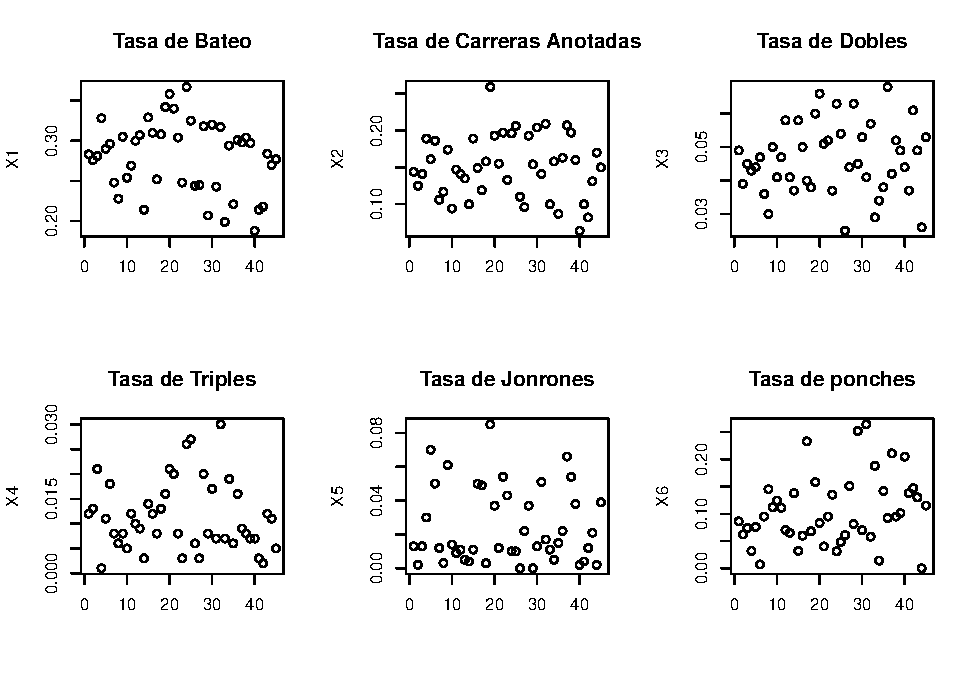
\includegraphics{Dispersion-y-Matriz-de-Correlacion_files/figure-latex/unnamed-chunk-3-1.pdf}

 \hypertarget{matriz-de-correlaciuxf3n}{%
 \subsection{Matriz de Correlación:}\label{matriz-de-correlaciuxf3n}}

 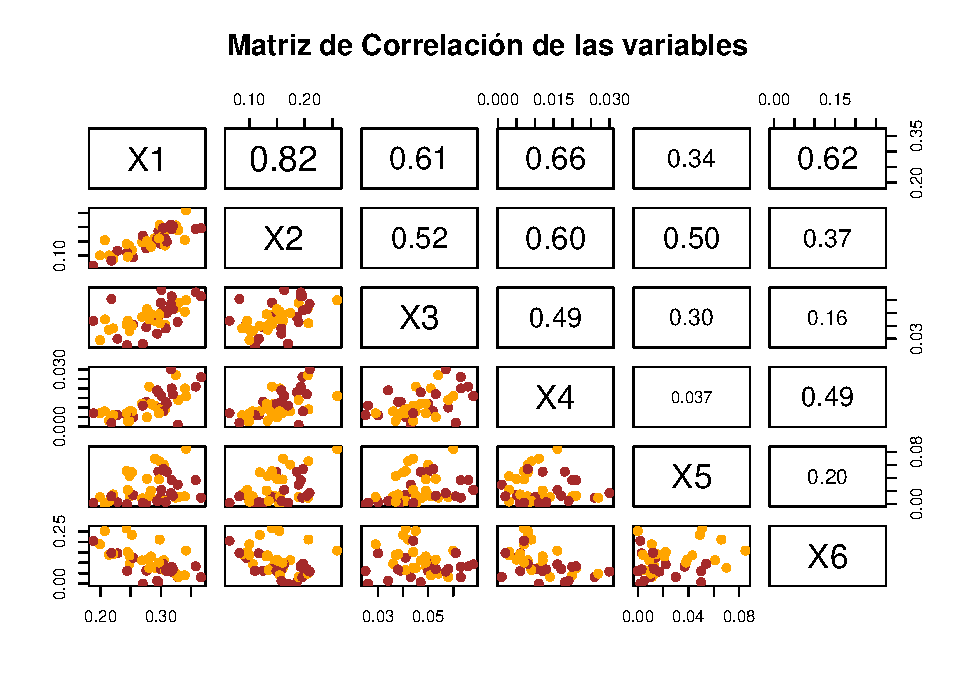
\includegraphics{Dispersion-y-Matriz-de-Correlacion_files/figure-latex/unnamed-chunk-4-1.pdf}
	
	%%%%%%%%%%%%% Fin del documento
	
	%%%%%%%%%%%% Inicio de la bibliografia
	
	\printbibliography
	
	
	%%%%%%%%%%%%% Fin de la bibliografia
	
	%%%%%%%%%%%%%%%%% Si hay cosas que incluir en include-after
		%%%%%%%%%%%%%%%%%%%%%%%%%%%%%%%%%%%%%%%%%%%%%%%%%%%%%%%%%%%%
	
\end{document}
